\documentclass[conference]{IEEEtran}
\usepackage{cite}
\usepackage{amsmath,amssymb}
\usepackage{graphicx}
\usepackage{booktabs}
\usepackage{url}
\def\UrlFont{\rmfamily}
\newtheorem{theorem}{Theorem}
\newtheorem{proposition}{Proposition}
\hyphenation{Puf-fer-fish de-hy-dra-tion re-hy-dra-tion}

\begin{document}

\title{DR-SL: Reversibility-Verified De-identification for Cloud-Local LLM Inference with Layered Assurance}

\author{\IEEEauthorblockN{Ya Yu\IEEEauthorrefmark{1}, Wen Hu\IEEEauthorrefmark{1}\IEEEauthorrefmark{2}, Xutong Wang\IEEEauthorrefmark{1}}
\IEEEauthorblockA{\IEEEauthorrefmark{1}College of Electronic and Information Engineering, Nanjing University of Aeronautics and Astronautics, Nanjing, China\\
\IEEEauthorrefmark{2}Jiangsu Yunhefeng Intelligent Technology Co., Ltd., Jiangsu, China\\
15949116139@163.com \quad huwen@nuaa.edu.cn \quad wsgxt@outlook.com}
\thanks{A preprint of an extended version of this work is available on arXiv (identifier to be inserted upon assignment). Code, synthetic datasets, the pre-registered experimental protocol, and the human-study packages are public at \texttt{https://gitee.com/jiangsu-yunhefeng-intelligent\_0/dr-sl} (code MIT; datasets CC-BY-4.0).}}

\maketitle

\begin{abstract}
Cloud-local LLM inference must keep sensitive user data on-device while exploiting cloud-grade reasoning, yet existing sanitizers---placeholder substitution, differential-privacy perturbation, and skill distillation---lack a release decision that is simultaneously safe and utility-preserving. We propose DR-SL (Dehydrate-Rehydrate with Self-Learning loop), which formalizes de-identification completeness as two measurable conditions---de-identification sufficiency under Pufferfish semantics and task-information preservation via QA probes---verified by a fully local two-branch loop under a lexicographic gate with guaranteed termination, backed by a deterministic hard line, an external strong-attacker re-test, and human fallback. We prove Fano-type leakage lower bounds, a Pufferfish witness, and a rate-privacy feasibility criterion, and state their scope plainly: the bounds certify leakage, never safety. On a worst-case fully task-coupled benchmark the loop reduces leakage $0.457\to0.304$ ($p\approx0$) and the release chain delivers $0.000$ literal leakage at egress (160 instances, two strong attackers); on a mixed-coupling benchmark the same safe point releases 67.5\% of instances automatically at zero measured leakage, Pareto-dominating placeholder and selective-LDP corners under an identical release rule. Two human studies anchor the semantic utility metric (Spearman $\rho=0.839$) and the annotation gold (type-level recall $\ge0.987$). The exploratory self-learning hypothesis was not supported and is reported as such.
\end{abstract}

\begin{IEEEkeywords}
sensitive-information isolation, cloud-local inference, dehydrate-rehydrate, reversibility verification, Pufferfish privacy, maximal leakage, prompt optimization
\end{IEEEkeywords}

\section{Introduction}

Cloud models reason better than on-device small models (SLMs), but forwarding requests exposes sensitive data; cloud-local systems~\cite{hao2024hybrid,siyan2025papillon} seek both, under the constraint that cloud-bound requests must exclude personally identifiable information (PII)~\cite{das2025security,lukas2023pii}. The open question is \emph{how to decide} that a cloud-bound artifact is safe: lax leaks, strict strips task semantics. A user typing ``I am 67, had a stent procedure at XX Hospital three months ago, and take aspirin daily; advise me on post-operative exercise'' is uniquely identifiable from the attribute combination alone~\cite{sweeney2002k}, yet deleting all details leaves the cloud unable to help.

Existing sanitizers fall into three classes, each defective. \emph{Entity-level placeholder substitution}~\cite{presidio,rehydra,zeng2025privacyrestore} covers only declared identifiers, misses semantic/quasi-identifier leakage, and destroys task context. \emph{Differential-privacy perturbation}~\cite{mai2023split,shi2022selective,duchi2013local} protects by noise that inherently degrades semantic coherence. \emph{Skill distillation} (P2Skill)~\cite{ryu2026p2skill} is closest to our setting, but its refinement loop requires the cloud, in reference and evaluator roles, to read PII-bearing original inputs (\cite{ryu2026p2skill}, \S3.3, steps 2--3; \S4.1), so refinement data must leave the device before refinement completes (its deployment-phase egress is matcher-gated); its matcher also covers only declared identifiers. All three are one-shot pipelines without cross-instance reuse or self-improvement.

We propose \textbf{DR-SL} (Dehydrate-Rehydrate with Self-Learning loop), which makes ``is de-identification complete?'' a measured, fully local decision (Fig.~\ref{fig:overview}): nothing leaves the device before the decision; a lexicographic iteration trades leakage against a utility gate with guaranteed termination; and a mandatory release chain (local gate $\to$ deterministic hard-line scrub $\to$ external strong-attacker re-test) decides egress, with INFEASIBLE instances routed to human review with residual-leakage reports. Contributions:
\begin{itemize}
\item A two-branch \emph{reversibility-verification} framework covering de-identification sufficiency (Pufferfish semantics, incl.\ quasi-identifier leakage) and task-information preservation (QA probes, incl.\ over-redaction detection), with a runtime cascade extractor and a recall-ceiling analysis delimiting the guarantee;
\item Theoretical positioning: a Fano-type lower bound on leakage from measured hit rates (the score certifies leakage, never safety), a Pufferfish witness, a rate-privacy feasibility criterion explaining inherent infeasibility, and a termination theorem;
\item A layered assurance model (calibrated soft certificate $+$ deterministic hard line $+$ human fallback) with a fully local self-learning loop, evaluated under a pre-registered protocol including two human studies and honestly reported negative self-learning results.
\end{itemize}

\begin{figure*}[!t]
\centering
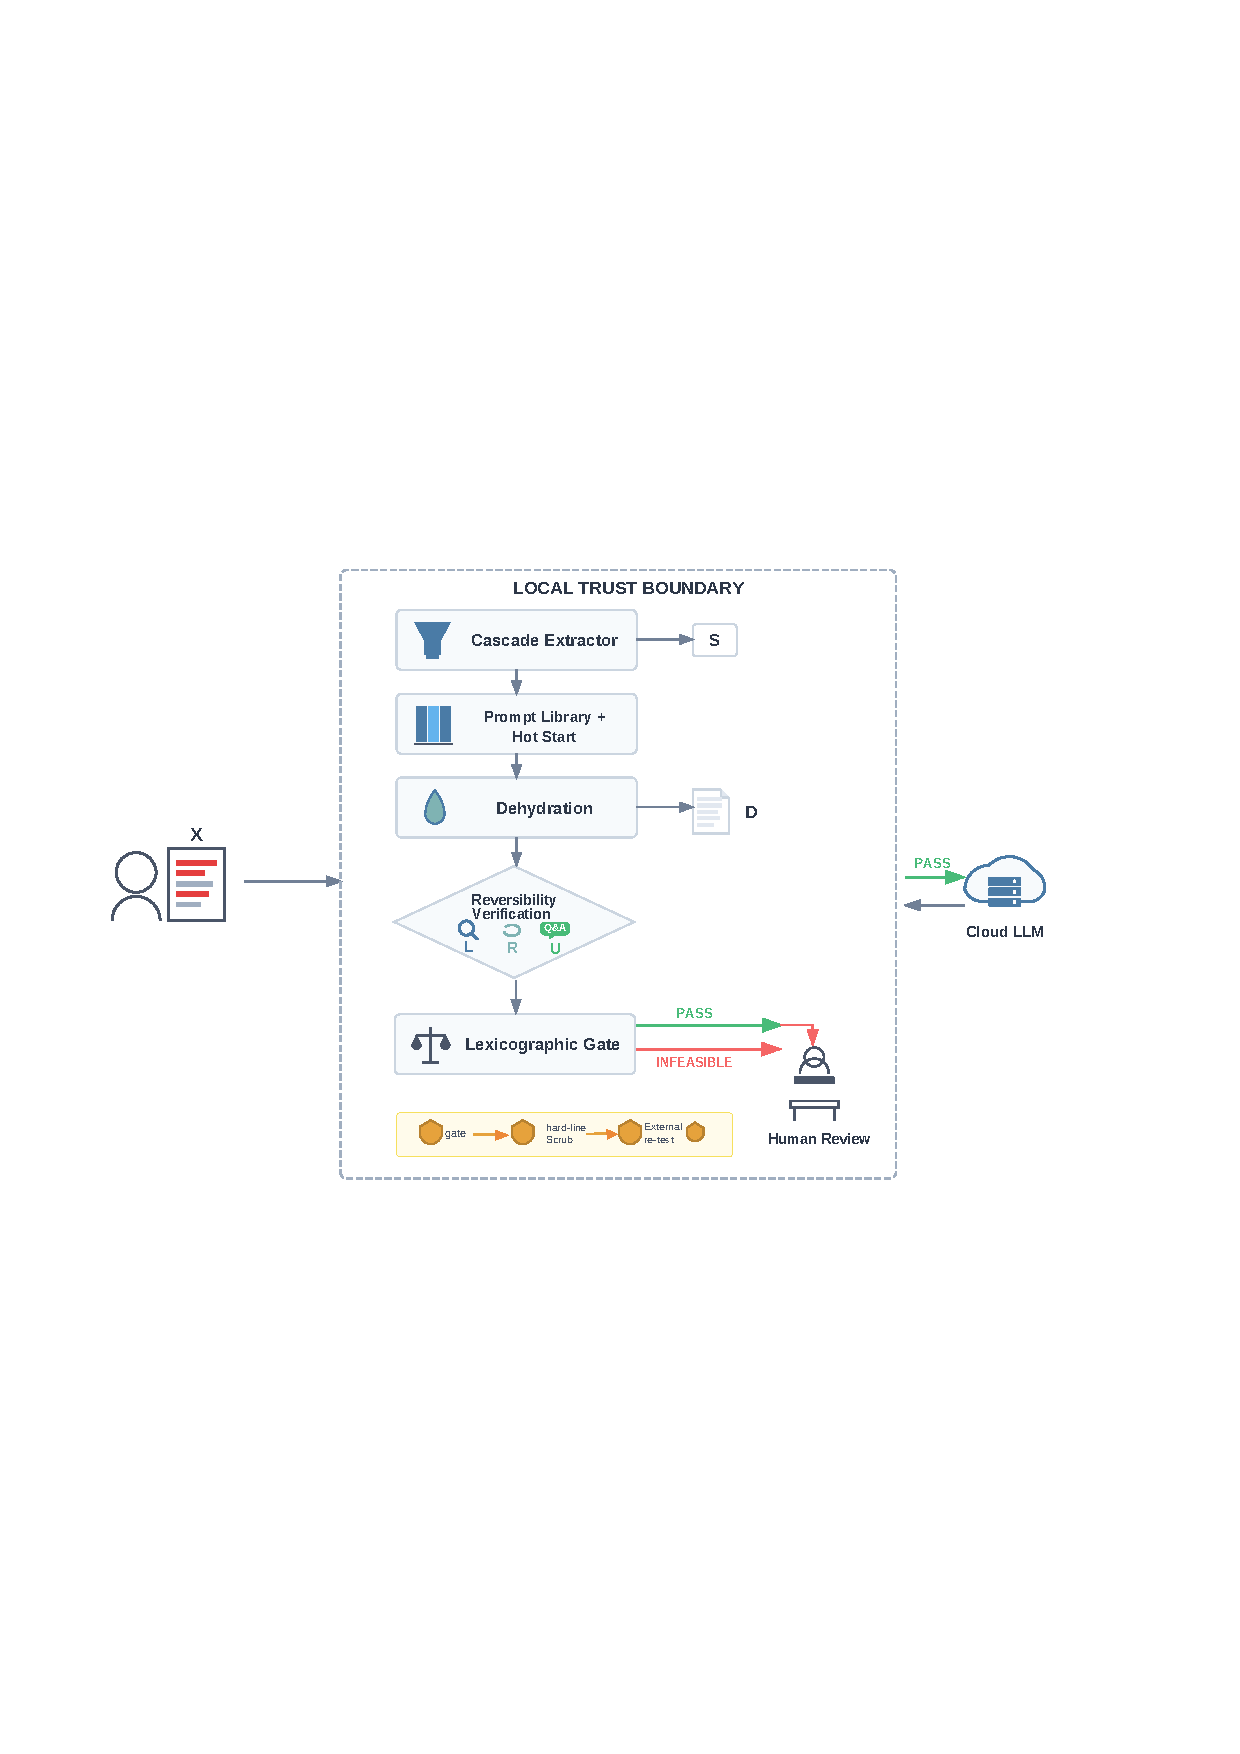
\includegraphics[width=0.62\textwidth,trim={49.3pt 271.9pt 89.2pt 269.2pt},clip]{figures/fig1.pdf}
\caption{DR-SL overview. Inside the local trust boundary, the cascade extractor derives the sensitive set $S$ from the original material $X$; a type-matched prompt library hot-starts dehydration into artifact $D$; two-branch reversibility verification (re-identification probes $L$, restoration $R$, QA utility probes $U$) feeds the lexicographic gate; the mandatory release chain (local gate $\to$ deterministic hard-line scrub $\to$ external strong-attacker re-test) decides egress: PASS sends only $D$ to the cloud LLM; INFEASIBLE emits a residual-leakage report and routes to human review. The re-test stage belongs to the destination trust class; only $D$ crosses the boundary.}
\label{fig:overview}
\end{figure*}

\section{Method}

\subsection{Formalization}

Let $X$ be the original material, $S=\{s_1,\dots,s_n\}$ the sensitive set (explicit identifiers or quasi-identifiers, each with domain $V_i$), $A$ attacker auxiliary knowledge, $T$ the task-relevant variable, and $D=\mathcal{D}(X)$ the dehydrated artifact. \emph{De-identification sufficiency} adopts Pufferfish semantics~\cite{kifer2012rigorous,kifer2014pufferfish}: with secrets $\sigma_{i,v}:=``s_i=v\text{''}$ and discriminative pairs $\mathcal{Q}$ (same-attribute distinct-value and identity pairs), the mechanism $P(D\mid X)$ satisfies $(\varepsilon,\mathcal{Q},\Theta)$-sufficiency iff for all $(\sigma,\sigma')\in\mathcal{Q}$, $\theta\in\Theta$, outputs $d$:
\begin{equation}
e^{-\varepsilon} \le \frac{P(D=d\mid \sigma,\theta)}{P(D=d\mid \sigma',\theta)} \le e^{\varepsilon}.
\label{eq:pufferfish}
\end{equation}
\emph{Task-information preservation} maximizes $I(D;T)$, measured operationally by a QA-probe utility $U$; the rehydration score $R$ (similarity of $\hat X$ reconstructed from $(D,S)$ to $X$) is a secondary diagnostic. Operationally, de-identification is \emph{complete} iff the Wilson-interval upper bound~\cite{wilson1927} of the leakage score $L$ satisfies $L\le\tau_L$ and $U\ge\tau_U$, conditioned on extractor recall $\hat\rho$ and attacker class $A_3$.

\subsection{Cascade Extractor and Recall Ceiling}

At runtime $S$ is produced by a cascade: (a) a regex/NER high-precision layer for explicit identifiers; (b) a local-LLM high-recall layer with a self-critique pass for quasi-identifiers; (c) a combination layer emitting quasi-identifier combinations for combination probes and $k$-anonymity tests~\cite{sweeney2002k}. Since Branch~1 probes only extracted attributes, missed attributes are never probed:

\begin{proposition}[Recall ceiling, over-extraction-corrected]
With gold set $G$, found set $F$, measured hit rate $L_{\mathrm{measured}}$ over $F$, and $\mathrm{Recall}=|F\cap G|/|G|$,
$L_{\mathrm{system}} \le (|F|/|G|)\,L_{\mathrm{measured}} + (1-\mathrm{Recall})$.
\end{proposition}

All system-level conclusions are therefore stated conditionally on measured recall $\hat\rho$ and inflation $\iota=|F|/|G|$ (on our data $\hat\rho=0.951$, $\iota=1.43$).

\subsection{Two-Branch Reversibility Verification}

\emph{Branch 1 (re-identification).} A local evaluator seeing only $D$ answers $\ge75$ probes built from $S$; per-attribute hit rates give $L=\frac{1}{|S|}\sum_i L_i$, and the gate uses the 95\% Wilson upper bound of $L$ against $\tau_L$ (resolving small-$|S|$ binomial granularity). Auxiliary knowledge is operationalized as nested attackers $A_0$ (general knowledge) $\subseteq A_1$ (domain priors) $\subseteq A_2$ (public retrieval) $\subseteq A_3$ (linkage database: synthetic-population $k$ counting, hit iff $k\le k^{*}{=}5$); non-monotone $L(A_i)$ triggers review. \emph{Branch 2 (rehydration, diagnostic).} From $(D,S)$ reconstruct $\hat X$; $R=\mathrm{Sim}(\hat X,X)$. \emph{Utility.} Task questions $Q_T$ generated from $X$ are answered from $X$ (reference) and from $D$ (target, same model and sampling---the deployment condition); $U$ is the mean agreement under exact/tolerance or rubric scoring.

\subsection{Lexicographic Iteration and Release Chain}

Same-round bidirectional updates can oscillate; DR-SL instead runs \emph{lexicographic} optimization: Phase~1 loosens dehydration until $U\ge\tau_U$ (no-progress exit after two failed loosens); Phase~2 repeatedly strengthens the highest-leak-contributing single attribute, accepting a step only if $U\ge\tau_U$ holds (hard gate), with one compensatory-loosen chance per attribute and permanent skipping otherwise; a hard budget $B=3|S|+5$ guarantees termination. Output is PASS($D$) with a stability window, or INFEASIBLE with a residual-leakage report (egress refused; human review). Because a local pass is only a lower-bound witness (Thm.~1), PASS is necessary but not sufficient for release: the mandatory chain is local gate $\to$ deterministic hard-line scrub (every declared literal removed or generalized, model-independent) $\to$ external strong-attacker re-test of the final artifact (a controlled first disclosure to the destination trust class) $\to$ egress or human review.

\section{Theoretical Properties}

Grading: theorems carry full proofs in the extended preprint; space permits statements and scope.

\begin{theorem}[Lower-boundedness of the leakage score, Fano-type]
If an attacker achieves per-attribute hit rate $L_i\ge 1/|V_i|$ on $s_i$, then
$I(D;S) \ge H(S) - \sum_i [H_2(1-L_i) + (1-L_i)\log(|V_i|-1)]$.
\end{theorem}

Measured attack success lower-bounds true leakage; a local evaluator's failure to re-identify cannot prove safety. We state the limit of this certificate: at $\tau_L=0.05$ with $|V|=100$, passing certifies only $\approx0.06$ bits ($\approx1\%$ of $H(s)$); for open-domain quasi-identifiers ($|V|\sim10^4$) $\approx0.34$ bits---near-vacuous. Safety therefore rests on empirical calibration $\hat\Delta=L_{\mathrm{cloud}}-L_{\mathrm{local}}$ (measured on non-sensitive corpora; $\hat\Delta=+0.181$ here), the hard line, and human fallback; Thm.~1 serves to witness leakage for rejection and warning.

\begin{proposition}[Pufferfish witness]
If the optimal attacker's hit rate on $s_i$ is $L$, with prior extremes $p_{\min},p_{\max}$, then any mechanism satisfying \eqref{eq:pufferfish} needs $\varepsilon \ge \ln\frac{L}{1-L} + \ln\frac{p_{\min}}{p_{\max}}$ (uniform prior: $\varepsilon\ge\ln\frac{L}{1-L}$).
\end{proposition}

\begin{proposition}[Feasibility criterion]
For any dehydrator, $I(D;T) \le I(D;S) + I(X;T\mid S)$; hence the rate-privacy function $U^{*}(\varepsilon)=\max_{I(D;S|A)\le\varepsilon} I(D;T) \le \varepsilon + I(X;T\mid S)$.
\end{proposition}

If $\tau_U > \tau_L + I(X;T\mid S)$ the feasible region is empty and the loop necessarily returns INFEASIBLE: infeasibility is a property of the problem (strong task--sensitive coupling), not a method defect.

\begin{theorem}[Termination]
The lexicographic iteration terminates in finitely many rounds with PASS or INFEASIBLE; after Phase~1 every accepted step maintains $U\ge\tau_U$.
\end{theorem}

\textbf{Layered assurance.} (1) \emph{Soft layer}: the calibrated certificate $\hat L = L_{\mathrm{local}}+\hat\Delta$, $U$, and $k$---quantitative, auditable, strengthening with evaluator capability; (2) \emph{hard line}: deterministic scrubbing of declared identifiers before egress, model-independent; (3) \emph{human fallback}: INFEASIBLE $\to$ residual report $\to$ human risk judgment. Each layer's guarantee and residual risk are explicitly statable; a compromised local device voids all guarantees (the threat model concerns the cloud/link adversary).

\section{Experiments}

\textbf{Setup.} A four-domain synthetic benchmark (medical/banking/travel/legal; all values fictional) isomorphic to P2Skill's 160-prompt PRISM set~\cite{ryu2026p2skill}: test-160 plus a 240-instance extension (100/domain), calibration 290 (non-sensitive by construction), train-400 online stream, adversarial 80, and a mixed-coupling set of 120 (mean coupling ratio 0.40: only task-critical types annotated task-relevant). Medical stems derive from MIT-licensed MedQA exam questions with all concrete values replaced~\cite{jin2021medqa}. Gates frozen pre-experiment: $\tau_L=0.05$ (Wilson semantics), $\ge75$ probes/instance, $\tau_U$ per metric; local executor ornith-1.5-35b; strong attackers/judges qwen3.8-max/flash and cross-family glm-5.2. All stages ran under a pre-registered protocol with a public deviation log (D1--D18); statistics use Wilson intervals, permutation and bootstrap tests.

\textbf{Extraction and annotation reliability.} Cascade recall is 0.951 overall (explicit 0.977, quasi 0.931; regex layer alone 97.4\% on regexable types but 46.1\% overall, confirming the cascade's necessity), with conservative over-extraction ($\iota=1.43$). Cross-family re-extraction (glm-5.2) reaches recall 0.983 (value-level Jaccard 0.79--0.85 across three architectures). A two-rater human audit of 50 instances validates the automatic gold (type-level recall 1.000/0.987, precision 0.959/0.991; combination-risk $\kappa=0.696$ under a construct-matched gold, residual divergences analysed and conservative).

\textbf{Main loop.} On train-400 under real gates, paired leakage falls $0.457\to0.304$ (permutation $p\approx0$, including INFEASIBLE) with PASS rate 37.5\% and the utility gate intact; on test-160 the loop reaches $L=0.436/0.412$ (flash/glm) from $0.768/0.789$ direct ($\approx45\%$ relative reduction, consistent across families; retrieval-augmented $A_2$ gains nothing on dehydrated text). An audit of archived loop outputs found 159/160 artifacts still carrying residual literals (mean 3.01/instance): utility measured pre-hard-line ($U\approx0.97$) was partly carried by those literals, a scope we state and correct below. After the deterministic hard-line scrub, \emph{literal leakage at egress is $0.000$} on all 160 instances under two strong attackers ($\ge75$ strict probes each; pooled 95\% upper bound $<0.001$)---the hard line, not the soft certificate, carries this guarantee; the scope is strict literal grading over declared attributes, not zero semantic leakage. Under the exact-value utility metric on this fully coupled benchmark the post-scrub utility is 0.000, so the effective automatic-release rate is 0\%: every instance routes to human review with a certificate package---the empirical incarnation of Prop.~3.

\textbf{Operating points and utility.} Table~\ref{tab:plane} completes the leakage-utility plane on test-160. Principled generalization (every occurrence of every declared value generalized or removed; task-relevant values generalized to bands/categories) matches the placeholder corner's zero literal leakage at higher utility, and the reference-based semantic judge $U_{\mathrm{sem}}$ (validated below) places it at 0.431---$1.9\times$ placeholder and $2.3\times$ selective LDP at equal-or-better leakage. Selective LDP leaks more ($L\approx0.05$) at chance-level utility.

\begin{table}[!t]
\centering
\caption{Leakage-utility plane on test-160 (strict-literal $L$ by two strong attackers; $U$ exact-value, $U_{\mathrm{sem}}$ semantic).}
\label{tab:plane}
\small
\begin{tabular}{@{}lcccc@{}}
\toprule
Operating point & $L$ flash & $L$ glm & $U$ & $U_{\mathrm{sem}}$ \\
\midrule
Direct forwarding & 0.768 & 0.789 & 0.917 & 1.000 \\
\textbf{Principled generalization} & \textbf{0.000} & \textbf{0.000} & 0.033$^{\dagger}$ & \textbf{0.431} \\
Placeholder substitution & 0.000 & 0.000 & 0.000 & 0.228 \\
Selective LDP & 0.057 & 0.049 & 0.075 & 0.188 \\
\bottomrule
\end{tabular}
\\[2pt]
{\footnotesize $^{\dagger}$0.276 with the completed generalization lexicon (numeric bands).}
\end{table}

\textbf{Mixed-coupling benchmark.} Where coupling is partial, automatic release becomes non-degenerate (Table~\ref{tab:mixed}): the safe point releases 67.5\% of instances automatically (95\% Wilson [58.6, 75.6]) at zero measured literal leakage and $U_{\mathrm{sem}}=0.571$, Pareto-dominating both corners measured under the identical release rule (placeholder 58.3\%; selective LDP 25.0\% and failing the leakage gate, $L=0.070$). The per-instance split---not a corpus average---is the decision mechanism's output.

\begin{table}[!t]
\centering
\caption{Mixed-coupling benchmark ($n{=}120$): identical release rule ($L\le\tau_L$, $U_{\mathrm{sem}}\ge0.5$).}
\label{tab:mixed}
\small
\begin{tabular}{@{}lccc@{}}
\toprule
Operating point & $L$ & $U_{\mathrm{sem}}$ & auto-release \\
\midrule
\textbf{Principled generalization} & \textbf{0.000} & \textbf{0.571} & \textbf{67.5\%} \\
Placeholder substitution & 0.000 & 0.421 & 58.3\% \\
Selective LDP & 0.070 & 0.254 & 25.0\% \\
\bottomrule
\end{tabular}
\end{table}

\textbf{Human anchors.} Human study~1 (two raters, 160 blinded rows over four operating points) validates the semantic judge: inter-rater Krippendorff $\alpha=0.780$, row-level Spearman $\rho=0.839$ against automatic $U_{\mathrm{sem}}$ (pre-registered bar $\ge0.8$), identical operating-point ranking; humans rate the safe point 0.487, above the automatic 0.406 on the same subset. The two raters are co-authors (Y. Yu and X. Wang), independent of the pipeline implementation and blind to variant identities.

\textbf{Self-learning (honest negative results).} Distilling 172 failure experiences into five prompt rules changed validation rounds from 2.82 to 2.90 ($p=0.68$): H1 (loop-count decrease) is \emph{not supported}---rules about recognition strategies are mechanistically decoupled from the loop's dehydration actions. The corrected hypothesis H1$'$ (rules targeting the extractor) raises quasi-identifier recall $0.928\to0.943$ ($+1.5$pp, one-sided $p=0.059$): directionally consistent, not significant at the pre-registered $p<0.05$. Both are reported as pre-registered outcomes.

\textbf{Probe format is a first-class factor.} The post-dehydration local-vs-strong gap ($\hat\Delta_{\mathrm{post}}\approx0.44$) is largely a probe-format artifact: under an enumeration prompt the local model lists residual literals it ``missed'' adversarially (recall 0.992). Re-running the full loop with the enumeration probe lowers PASS from 43.8\% to 5.0\% (false passes become strengthening or honest INFEASIBLE routing) and \emph{increases} the measured paired reduction ($-0.404$ vs $-0.154$ on train-400): the headline reduction is robust to probe format, while open-vocabulary categorical residuals remain for the hard line and re-test.

\textbf{Limitations.} Certificate strength is bounded by evaluator capability and calibration transfer; guarantees are conditioned on $\hat\rho$ and attacker class $A_3$; strongly coupled tasks admit no non-degenerate automatic point (Prop.~3); the $\ge75$-probe gate costs $\approx203$--240\,s/instance.

\section{Conclusion}

DR-SL turns ``is de-identification complete?'' into a measured local decision with Pufferfish semantics, QA-probe utility, a terminating lexicographic loop, and a layered release chain whose deterministic and human layers carry the egress guarantee the soft certificate honestly cannot. Experiments under a pre-registered protocol quantify leakage reduction, zero literal egress leakage, the leakage-utility frontier, where automatic release is non-degenerate, and two human anchors---alongside unsupported self-learning hypotheses reported as such. Future work includes powered H1$'$ re-tests, computable Maximal-Leakage upper bounds, real-statistics $k$ populations, larger human studies, and interactive-latency engineering.

\begin{thebibliography}{24}
\bibitem{hao2024hybrid} H. Hao, H. Jiang, S. Jiang, J. Ren, and T. Cao, ``Hybrid SLM and LLM for edge-cloud collaborative inference,'' in \emph{Workshop on Edge and Mobile Foundation Models (EdgeFM)}, 2024, pp. 36--41.
\bibitem{siyan2025papillon} L. Siyan, V. C. Raghuram, O. Khattab \emph{et al.}, ``PAPILLON: privacy preservation from internet-based and local language model ensembles,'' in \emph{NAACL}, 2025.
\bibitem{das2025security} B. C. Das, M. H. Amini, and Y. Wu, ``Security and privacy challenges of large language models: a survey,'' \emph{ACM Comput. Surv.}, vol. 57, no. 6, pp. 1--39, 2025.
\bibitem{lukas2023pii} N. Lukas, A. Salem, R. Sim \emph{et al.}, ``Analyzing leakage of personally identifiable information in language models,'' in \emph{IEEE S\&P}, 2023.
\bibitem{presidio} data-privacy-stack, ``Presidio: open-source framework for detecting, redacting, and anonymizing PII,'' GitHub.
\bibitem{rehydra} rehydra-ai, ``Rehydra SDK: PII security for AI workflows,'' GitHub, MIT.
\bibitem{zeng2025privacyrestore} Z. Zeng, J. Wang, J. Yang \emph{et al.}, ``PrivacyRestore: privacy-preserving inference in large language models via privacy removal and restoration,'' in \emph{ACL}, 2025.
\bibitem{mai2023split} P. Mai, R. Yan, Z. Huang, Y. Yang, and Y. Pang, ``Split-and-denoise: protect large language model inference with local differential privacy,'' arXiv:2310.09130, 2023.
\bibitem{shi2022selective} W. Shi, A. Cui, E. Li \emph{et al.}, ``Selective differential privacy for language modeling,'' in \emph{NAACL}, 2022.
\bibitem{duchi2013local} J. C. Duchi, M. I. Jordan, and M. J. Wainwright, ``Local privacy and statistical minimax rates,'' in \emph{IEEE FOCS}, 2013, pp. 429--438.
\bibitem{ryu2026p2skill} M. Ryu, G. Park, S. Lee, X. Piao, and J. Kim, ``P2Skill: privacy preserving skill distillation for cloud-local LLM inference systems,'' arXiv:2608.14094, 2026.
\bibitem{kifer2012rigorous} D. Kifer and A. Machanavajjhala, ``A rigorous and customizable framework for privacy,'' in \emph{PODS}, 2012, pp. 77--88.
\bibitem{kifer2014pufferfish} D. Kifer and A. Machanavajjhala, ``Pufferfish: a framework for mathematical privacy definitions,'' \emph{ACM Trans. Database Syst.}, vol. 39, no. 1, pp. 3:1--3:36, 2014.
\bibitem{issa2020operational} I. Issa, A. B. Wagner, and S. Kamath, ``An operational approach to information leakage,'' \emph{IEEE Trans. Inf. Theory}, vol. 66, no. 3, pp. 1625--1657, 2020.
\bibitem{sweeney2002k} L. Sweeney, ``$k$-anonymity: a model for protecting privacy,'' \emph{Int. J. Uncertainty, Fuzziness Knowl.-Based Syst.}, vol. 10, no. 5, pp. 557--570, 2002.
\bibitem{wilson1927} E. B. Wilson, ``Probable inference, the law of succession, and statistical inference,'' \emph{JASA}, vol. 22, no. 158, pp. 209--212, 1927.
\bibitem{fabbri2022qafacteval} A. R. Fabbri, C. Wu, W. Liu, and C. Xiong, ``QAFactEval: improved QA-based factual consistency evaluation for summarization,'' in \emph{NAACL-HLT}, 2022, pp. 2587--2601.
\bibitem{pilan2025truthful} I. Pil\'an, B. Manzanares-Salor, D. S\'anchez, and P. Lison, ``Truthful text sanitization guided by inference attacks,'' \emph{Appl. Soft Comput.}, vol. 185, p. 114013, 2025.
\bibitem{jin2021medqa} Q. Jin, B. Dhingra, Z. Liu, W. W. Cohen, and X. Lu, ``What disease does this patient have? A large-scale open domain question answering dataset from medical exams,'' \emph{Appl. Sci.}, vol. 11, no. 14, p. 6421, 2021.
\bibitem{ornith35b} ornith-ai, ``Ornith-1.5-35B-A3B,'' Hugging Face, 2026.
\bibitem{qwen3827b} Qwen, ``Qwen3.8-27B,'' Hugging Face, 2026.
\end{thebibliography}

\end{document}
